% !TeX program = xelatex
\documentclass[10pt,a4paper]{ctexart} % 设置文章类型，正文字号与纸张大小

% 页面与正文常用宏包
\usepackage[margin=2cm]{geometry} % 设置页面四周页边距
\usepackage{graphicx}             % 插入图片
\usepackage{amsmath}              % 提供cases、aligned等数学公式环境
\usepackage{amssymb}              % 提供\therefore等扩展数学符号
\usepackage{booktabs}             % 提供\toprule、\midrule、\bottomrule三线表命令
\usepackage{float}                % 提供[H]固定图片、表格位置
\usepackage{subcaption}           % 提供subfigure子图环境及子图标题
\usepackage{wrapfig}              % 提供wrapfigure图文环绕环境
\usepackage{fancyhdr}             % 自定义页眉和页脚
\usepackage{hyperref}             % 生成超链接

% 页眉页脚
\pagestyle{fancy}                  % 启用fancyhdr定义的页面样式
\fancyhf{}                         % 清空默认页眉和页脚
\fancyfoot[C]{\thepage}            % 在页脚中央显示页码
\renewcommand{\headrulewidth}{0pt} % 隐藏页眉横线
\renewcommand{\footrulewidth}{0pt} % 隐藏页脚横线

% 超链接
\hypersetup{
  colorlinks=true,                % 使用彩色文字链接，而非带边框的链接
  linkcolor=red,                 % 目录、公式及图表交叉引用的颜色
  filecolor=cyan,                 % 本地文件链接的颜色
  urlcolor=blue,                  % 网址链接的颜色
  pdftitle={密立根油滴实验预习报告},     % 写入PDF文档属性的标题
  bookmarksnumbered=true          % PDF书签显示章节编号
}

% 定义字号命令
\newcommand{\chuhao}{\fontsize{42pt}{63pt}\selectfont}
\newcommand{\xiaochu}{\fontsize{36pt}{54pt}\selectfont}
\newcommand{\yihao}{\fontsize{26pt}{39pt}\selectfont}
\newcommand{\xiaoyi}{\fontsize{24pt}{36pt}\selectfont}
\newcommand{\erhao}{\fontsize{22pt}{33pt}\selectfont}
\newcommand{\xiaoer}{\fontsize{18pt}{27pt}\selectfont}
\newcommand{\sanhao}{\fontsize{16pt}{24pt}\selectfont}
\newcommand{\xiaosan}{\fontsize{15pt}{22.5pt}\selectfont}
\newcommand{\sihao}{\fontsize{14pt}{21pt}\selectfont}
\newcommand{\xiaosi}{\fontsize{12pt}{18pt}\selectfont}
\newcommand{\wuhao}{\fontsize{10.5pt}{15.75pt}\selectfont}
\newcommand{\xiaowu}{\fontsize{9pt}{13.5pt}\selectfont}

% 章节格式
\ctexset{
  section={
    format={\CJKfontspec[AutoFakeBold=2.5]{KaiTi}\sanhao\bfseries}, % 一级标题使用三号加粗楷体
    name={,、},                                                    % 在中文章节序号后添加顿号
    number=\chinese{section},                                      % 一级标题编号使用“一、二、三”形式
    aftername={}                                                   % 取消编号与标题文字之间的空格
  },
  subsection={
    format={\CJKfontspec[AutoFakeBold=2.5]{KaiTi}\sihao\bfseries}, % 二级标题使用四号加粗楷体
  },
  subsubsection={
    format={\CJKfontspec[AutoFakeBold=2.5]{KaiTi}\xiaosi\bfseries}, % 三级标题使用小四加粗楷体
  }
}

\begin{document}

% 封面
\thispagestyle{fancy} % 封面保留底部居中的页码
\fancyfoot[C]{\thepage}
\begin{center}
  \CJKfontspec[AutoFakeBold=2.5]{KaiTi}\bfseries % 封面中文使用楷体并人工加粗，西文同时加粗
  \vspace*{2.0cm}
  \xiaochu 
    物理实验预习报告

  \vspace{3.8cm}
  \begin{minipage}{10.0cm}
    \sanhao
    \makebox[2.6cm][l]{实验名称：}
    \underline{\makebox[7.0cm][c]{密立根油滴实验}}\par\vspace{12pt}

    \makebox[2.6cm][l]{指导老师：}
    \underline{\makebox[7.0cm][c]{郭红丽}}\par\vspace{12pt}
  \end{minipage}

  \vspace{3.8cm}
  \begin{minipage}{10.0cm}
    \sihao
    \makebox[1.4cm][l]{班级：}
    \underline{\makebox[8.0cm][c]{信工2503}}\par\vspace{10pt}

    \makebox[1.4cm][l]{姓名：}
    \underline{\makebox[8.0cm][c]{陈源}}\par\vspace{10pt}

    \makebox[1.4cm][l]{学号：}
    \underline{\makebox[8.0cm][c]{3250103617}}
  \end{minipage}

  \vspace{1.8cm}
  \sihao
    实验日期：
    \underline{\makebox[0.7cm][c]{2026}}年
    \underline{\makebox[0.7cm][c]{11}}月
    \underline{\makebox[0.7cm][c]{11}}日
    星期\underline{\makebox[0.7cm][c]{三}}上午

  \vspace{0.7cm}
  \sihao 
    浙江大学物理实验教学中心
\end{center}

\newpage
\xiaosi\songti\mdseries % 后续正文统一使用小四不加粗的宋体

\section{预习报告（10分）}

  \subsection{实验综述（5分）}
  
    \subsubsection{实验背景}
    \begin{wrapfigure}{r}{0.2\textwidth}
      \centering
      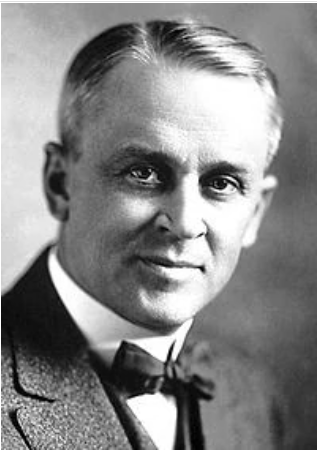
\includegraphics[width=\linewidth]{figures/图1.png}
      \caption{罗伯特·密立根（美国）}
    \end{wrapfigure}

    基本电荷值精确测量者：密立根。
    \begin{itemize}
      \item 密立根利用在电场和重力场中运动的带电油滴精确地测定了基本电荷。
      \item 基本电荷：电荷都是最小基本电荷的整数倍。
    \end{itemize}

    \subsubsection{静态平衡法}
    油滴在平板之间将同时受到重力和静电力的作用。
    
    通过调节板间电压，可以使两个力达到平衡。

    \begin{figure}[H]
      \centering
      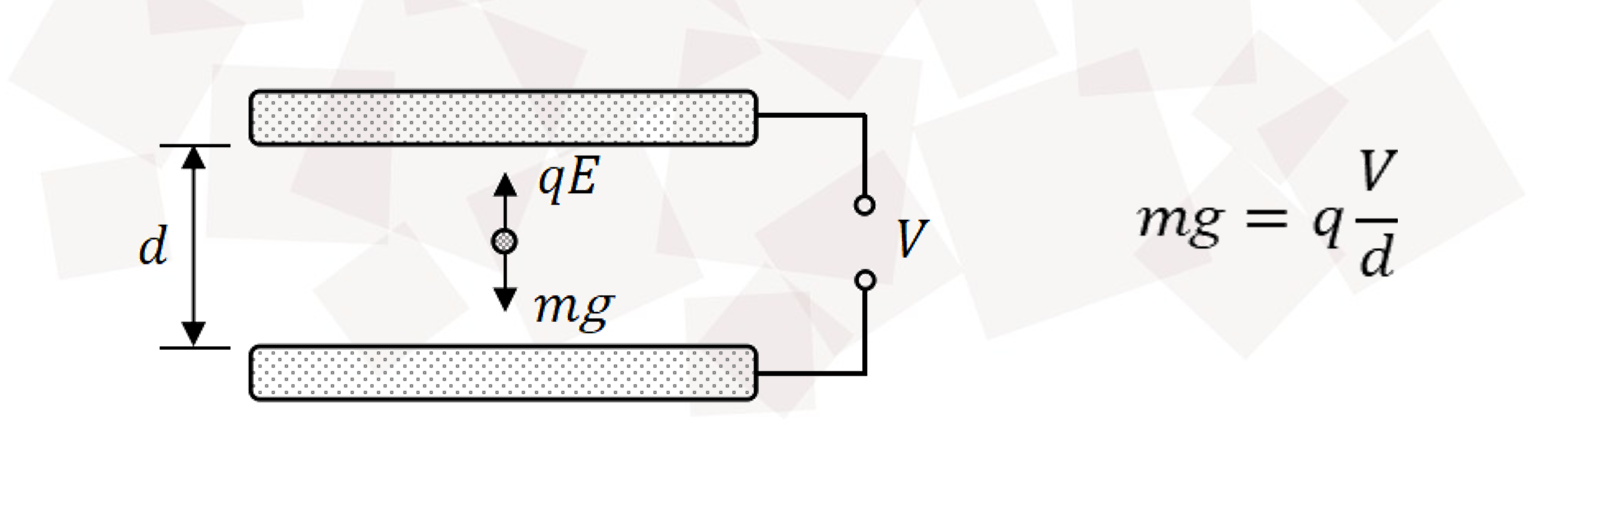
\includegraphics[width=0.75\textwidth]{figures/图2.png}
      \caption{重力与静电力平衡}
    \end{figure}

    \subsubsection{匀速下降法与油滴质量测定}
    设油滴呈小球状，当平板上未加电压时，油滴会加速下落，直到粘滞阻力与重力平衡而匀速下落。

    \[
    \left\{
    \begin{aligned}
    m &= \frac{4}{3}\pi r^3 \rho \\
    f &= 6\pi r\eta v = mg
    \end{aligned}
    \right.
    \quad\Longrightarrow\quad
    r = \sqrt{\frac{9\eta v}{2\rho g}}
    \quad\Longrightarrow\quad
    f = \frac{6\pi r\eta v}{1+\dfrac{b}{pr}}
    \]

    \[
    r
    = \sqrt{
    \frac{9\eta v}{2\rho g}
    \cdot
    \frac{1}{1+\dfrac{b}{pr}}
    }
    \]

    \subsubsection{基本电荷量测定}
    所有带电油滴所携带的电量均是最小电荷量的整数倍，这充分证明了电荷的不连续性。

    \[
    \left.
    \begin{aligned}
    mg &= q\frac{V}{d} \\[1em]
    v &= \frac{l}{t} \\[1em]
    r &= \sqrt{
        \frac{9\eta v}{2\rho g}
        \cdot
        \frac{1}{1+\dfrac{b}{pr}}
    }
    \end{aligned}
    \right\}
    \quad\Longrightarrow\quad
    q = \frac{18\pi}{\sqrt{2\rho g}}
        \left[
            \frac{\eta l}{t\left(1+\dfrac{b}{pr}\right)}
        \right]^{3/2}
        \frac{d}{V}
    \quad\Longrightarrow\quad
    q = mg\frac{d}{V_n} = ne
    \]

    \subsubsection{实验内容}
    主要分为如下两大步骤。
    \begin{enumerate}
      \item 练习找合适油滴
      
      油滴选取原则：应选择电量较小且质量适中的油滴。实验中，通常选取带电量小于10个基本电荷、平衡电压约200V、下落时间在10秒/毫米以内的清晰可见油滴。
      因此，需训练以寻找合适的油滴。若油滴带电量过大，相邻带电油滴将难以区分；若油滴带电量过小，质量也随之减小，更易受空气分子布朗运动的影响。
      
      \item 测量油滴基本电荷量
      \begin{enumerate}
         \item 选取合适油滴，调节电压使油滴悬浮。
         \item 多次测量同一油滴匀速下降的距离及其所用时间（也可使用不同的多颗油滴进行相同的测量）。
         \item 公约数法计算基本电荷量（也可以用其他数据处理方法）。
      \end{enumerate}
    \end{enumerate} 

  \subsection{实验重点（3分）}
  \begin{enumerate}
    \item 了解密立根油滴仪工作特性。
    \item 测定电子基本电荷量。
    \item 掌握密立根油滴实验数据处理方法。
  \end{enumerate}

  \subsection{实验难点（2分）}
  \begin{enumerate}
    \item 选择大小适中、清晰稳定且带电量合适的油滴进行测量；
    \item 准确调节平衡电压，并测量油滴匀速下落的距离和时间；
    \item 根据多次测量数据计算油滴电荷量，利用公约数法确定基本电荷量。
  \end{enumerate}

\vspace*{\fill} % 使下面内容在页面底部显示
\noindent
\begin{minipage}{\textwidth}
  注意事项：

  \begingroup
    \setlength{\leftskip}{2em} % 1--4整体向右缩进两个汉字宽度
    1. 用PDF格式上传“实验报告”，文件名：学生姓名+学号+实验名称+周次。

    2. “实验报告”必须递交在“学在浙大”本课程内对应实验项目的“作业”模块内。

    3. “实验报告”成绩必须在“浙江大学物理实验教学中心网站”-“选课系统”内查询。

    4. 教学评价必须在“浙江大学物理实验教学中心网站”-“选课系统”内进行，学生必须进行教学评价，才能看到实验报告成绩，教学评价须在本次实验结束之后3天内进行。\par
  \endgroup

  \begin{center}
    {\CJKfontspec[AutoFakeBold=2.5]{SimSun}\bfseries 浙江大学物理实验教学中心制}
  \end{center}
\end{minipage}

\end{document}

